\documentclass[]{article}
\usepackage[super,numbers]{natbib}

\usepackage[margin=1in]{geometry}
\usepackage{url}
\usepackage{graphicx}
\usepackage{color}
\usepackage{booktabs}

\usepackage{authblk}
\renewcommand{\Affilfont}{\normalsize}
\renewcommand{\Authfont}{\normalsize}

% local definitions
\newcommand{\comment}[1]{{\textcolor{red}{Co-author: #1}}}
\newcommand{\sgcomment}[1]{{\textcolor{red}{SG: #1}}}
\newcommand{\bmhcomment}[1]{{\textcolor{blue}{BMH: #1}}}
\newcommand{\aprcomment}[1]{{\textcolor{magenta}{APR: #1}}}
\newcommand{\tdwcomment}[1]{{\textcolor{cyan}{TDW: #1}}}

% cross-reference with supplement
\usepackage{xr}
\externaldocument{supplement}

\begin{document}

\title{A weakly structured stem for human origins in Africa}
\author[1]{Aaron P. Ragsdale}
\author[2]{Timothy D. Weaver}
\author[3]{Elizabeth G. Atkinson}
\author[4]{Eileen Hoal}
\author[4]{Marlo M\"{o}ller}
\author[2,5,$\dag$,*]{Brenna M. Henn}
\author[6,$\dag$,**]{Simon Gravel}
\affil[1]{Department of Integrative Biology, University of Wisconsin--Madison, WI, USA}
\affil[2]{Department of Anthropology, University of California, Davis, Davis, CA, USA}
\affil[3]{Department of Molecular and Human Genetics, Baylor College of Medicine, Houston, TX, USA}
\affil[4]{DSI-NRF Centre of Excellence for Biomedical Tuberculosis Research; South African Medical Research Council Centre for Tuberculosis Research; Division of Molecular Biology and Human Genetics, Faculty of Medicine and Health Sciences, Stellenbosch University, Cape Town, South Africa}
\affil[5]{UC Davis Genome Center, University of California, Davis, Davis, CA, USA}
\affil[6]{Department of Human Genetics, McGill University, Montreal, QC, Canada}
\affil[$\dag$]{Co-Corresponding Authors}
\affil[*]{bmhenn@ucdavis.edu}
\affil[**]{simon.gravel@mcgill.ca}
\date{\normalsize \today}
\maketitle

\begin{abstract}
While it is now broadly accepted that \emph{Homo sapiens}
originated within Africa, considerable
uncertainty surrounds specific models of divergence and migration across the
continent. Progress is hampered by a paucity of fossil and genomic data, as
well as variability in prior divergence time estimates.
Here we use linkage disequilibrium and
diversity-based statistics, optimized for rapid, complex demographic inference
to discriminate among such models.
We infer detailed demographic models for
populations across Africa, including representatives from eastern and western
groups, as well as 44 newly whole-genome sequenced individuals from the Nama
(Khoe-San). Despite the complexity of African population history, contemporary
population structure dates back to Marine Isotope Stage (MIS) 5. The earliest
population divergence among contemporary populations occurs 120-135ka, between
the Khoe-San and other groups. Prior to the divergence of contemporary African
groups, we infer long-lasting structure between two or more weakly
differentiated ancestral \emph{Homo}
populations connected by gene flow over
hundreds of thousands of years (i.e. a weakly structured stem). We find that
weakly structured stem models provide more likely explanations of polymorphism
that had previously been attributed to contributions from archaic hominins in
Africa.
In contrast to models with archaic introgression, we predict that fossil
remains from coexisting ancestral populations should be morphologically
similar.
Despite genetic similarity between these populations, an inferred 1--4\%
of genetic differentiation among contemporary human populations can be
attributed to genetic drift between stem populations.
We show that model misspecification explains variation in previous
divergence time estimates and argue that studying a suite of models is key to
robust inferences about deep history.
\end{abstract}

\section*{Introduction}


Decades of study of human genome variation have suggested a predominantly
tree-like model of recent population divergence from a single ancestral
population in Africa. It has been difficult to reconcile this finding with the
fossil and archaeological records of human occupation across the vast African
continent. For example, fossils such as those from the sites of Jebel Irhoud,
Morocco \citep{Hublin2017-cq}, Herto, Ethiopia \citep{White2003-bk} and Klasies
River, South Africa \citep{Deacon1995-rx} demonstrate that derived \emph{Homo
sapiens} anatomical features were intermittantly present across the continent
300-100ka. Archaeological sites from the Middle Stone Age, of which some have
been associated with \emph{Homo sapiens}, are also widely distributed across
Africa. It is unclear whether these fossils and archaeological sites represent
populations which contributed to contemporary \emph{Homo sapiens} as population
precedents or were local ``dead-ends''. Recently, attempts to reconcile genetic
and paleoanthropological data include proposals for a Pan-African origin of
\emph{Homo sapiens} by which populations in many regions of the continent
contributed to the formation of \emph{Homo sapiens} beginning at least 300ka
\citep{Stringer2016-mj,Scerri2018-nl,Scerri2019-xg}.

Genetic models have been hampered in their contribution to this discussion
because they primarily assume (or, at least, have been tested under) a
tree-like model of isolation-with-migration. Alternative theoretical scenarios
have been proposed, such as stepping stone models \citep{Arredondo2021-qa} or
population coalescence and fragmentation \citep{Scerri2019-xg}, but these
approaches are more challenging to interpret and fit to data.
However, new population genetic tools now allow for inference involving tens to
hundreds of genomes from multiple populations and greater complexity
\citep{Kamm2020-vn,Ragsdale2019-nt,Speidel2019-nj}. Inspired by evidence for
Neanderthal admixture with humans in Eurasia, several recent articles
have shown that introducing an archaic hominin ghost population contributing to African
populations in the period surrounding the Out-of-Africa migration event
substantially improves the description of genetic data relative to
single-origin models
\citep{Plagnol2006-lt,Hammer2011-bx,Hsieh2016-gk,Hey2018-pw,Ragsdale2019-nt,Lorente-Galdos2019-vz,Durvasula2020-td}.
This has driven speculation about the geographic range of this ghost
population, possible links to specific fossils, and the possibility of
finding ancient DNA evidence (e.g.\citep{Hsieh2016-gk}). However, these prior
articles share two weaknesses. First, they only contrast a single-origin model
with an archaic hominin admixture model, leaving out other plausible models
\citep{Henn2018-rf} (Figure~\ref{fig:proposed-models}).
Second, they
focus on a small subset of African diversity, either because of small sample
sizes (2-5 genomes) or because they rely on 1000 Genomes data which only
recruited populations of recent West African or Bantu-speaking ancestry
(Figure~\ref{fig:diversity}C). 
While ancient DNA from Eurasia has helped us understand early human history
outside of Africa, there is no comparably ancient DNA to elucidate early history
in Africa \citep{Lipson2022-xf}.

We therefore aim to discriminate among a broader set of demographic
models by studying the genomes of contemporary populations. We take as our
starting point four classes of models (single population expansion, single
population expansion with regional persistence, archaic hominin admixture, and
multi-regional evolution, Figure~\ref{fig:proposed-models}), using 290
genomes of individuals from southern, eastern, and western Africa as well as Eurasia. By
including geographically and genetically diverse populations across Africa, we
infer demographic models that explain more features of genetic diversity
in more
populations than previously reported. These analyses confirm the inadequacy of
tree-like models and provide an opportunity to directly evaluate a wide range
of alternative models. 


\begin{figure}[ht]
    \centering
    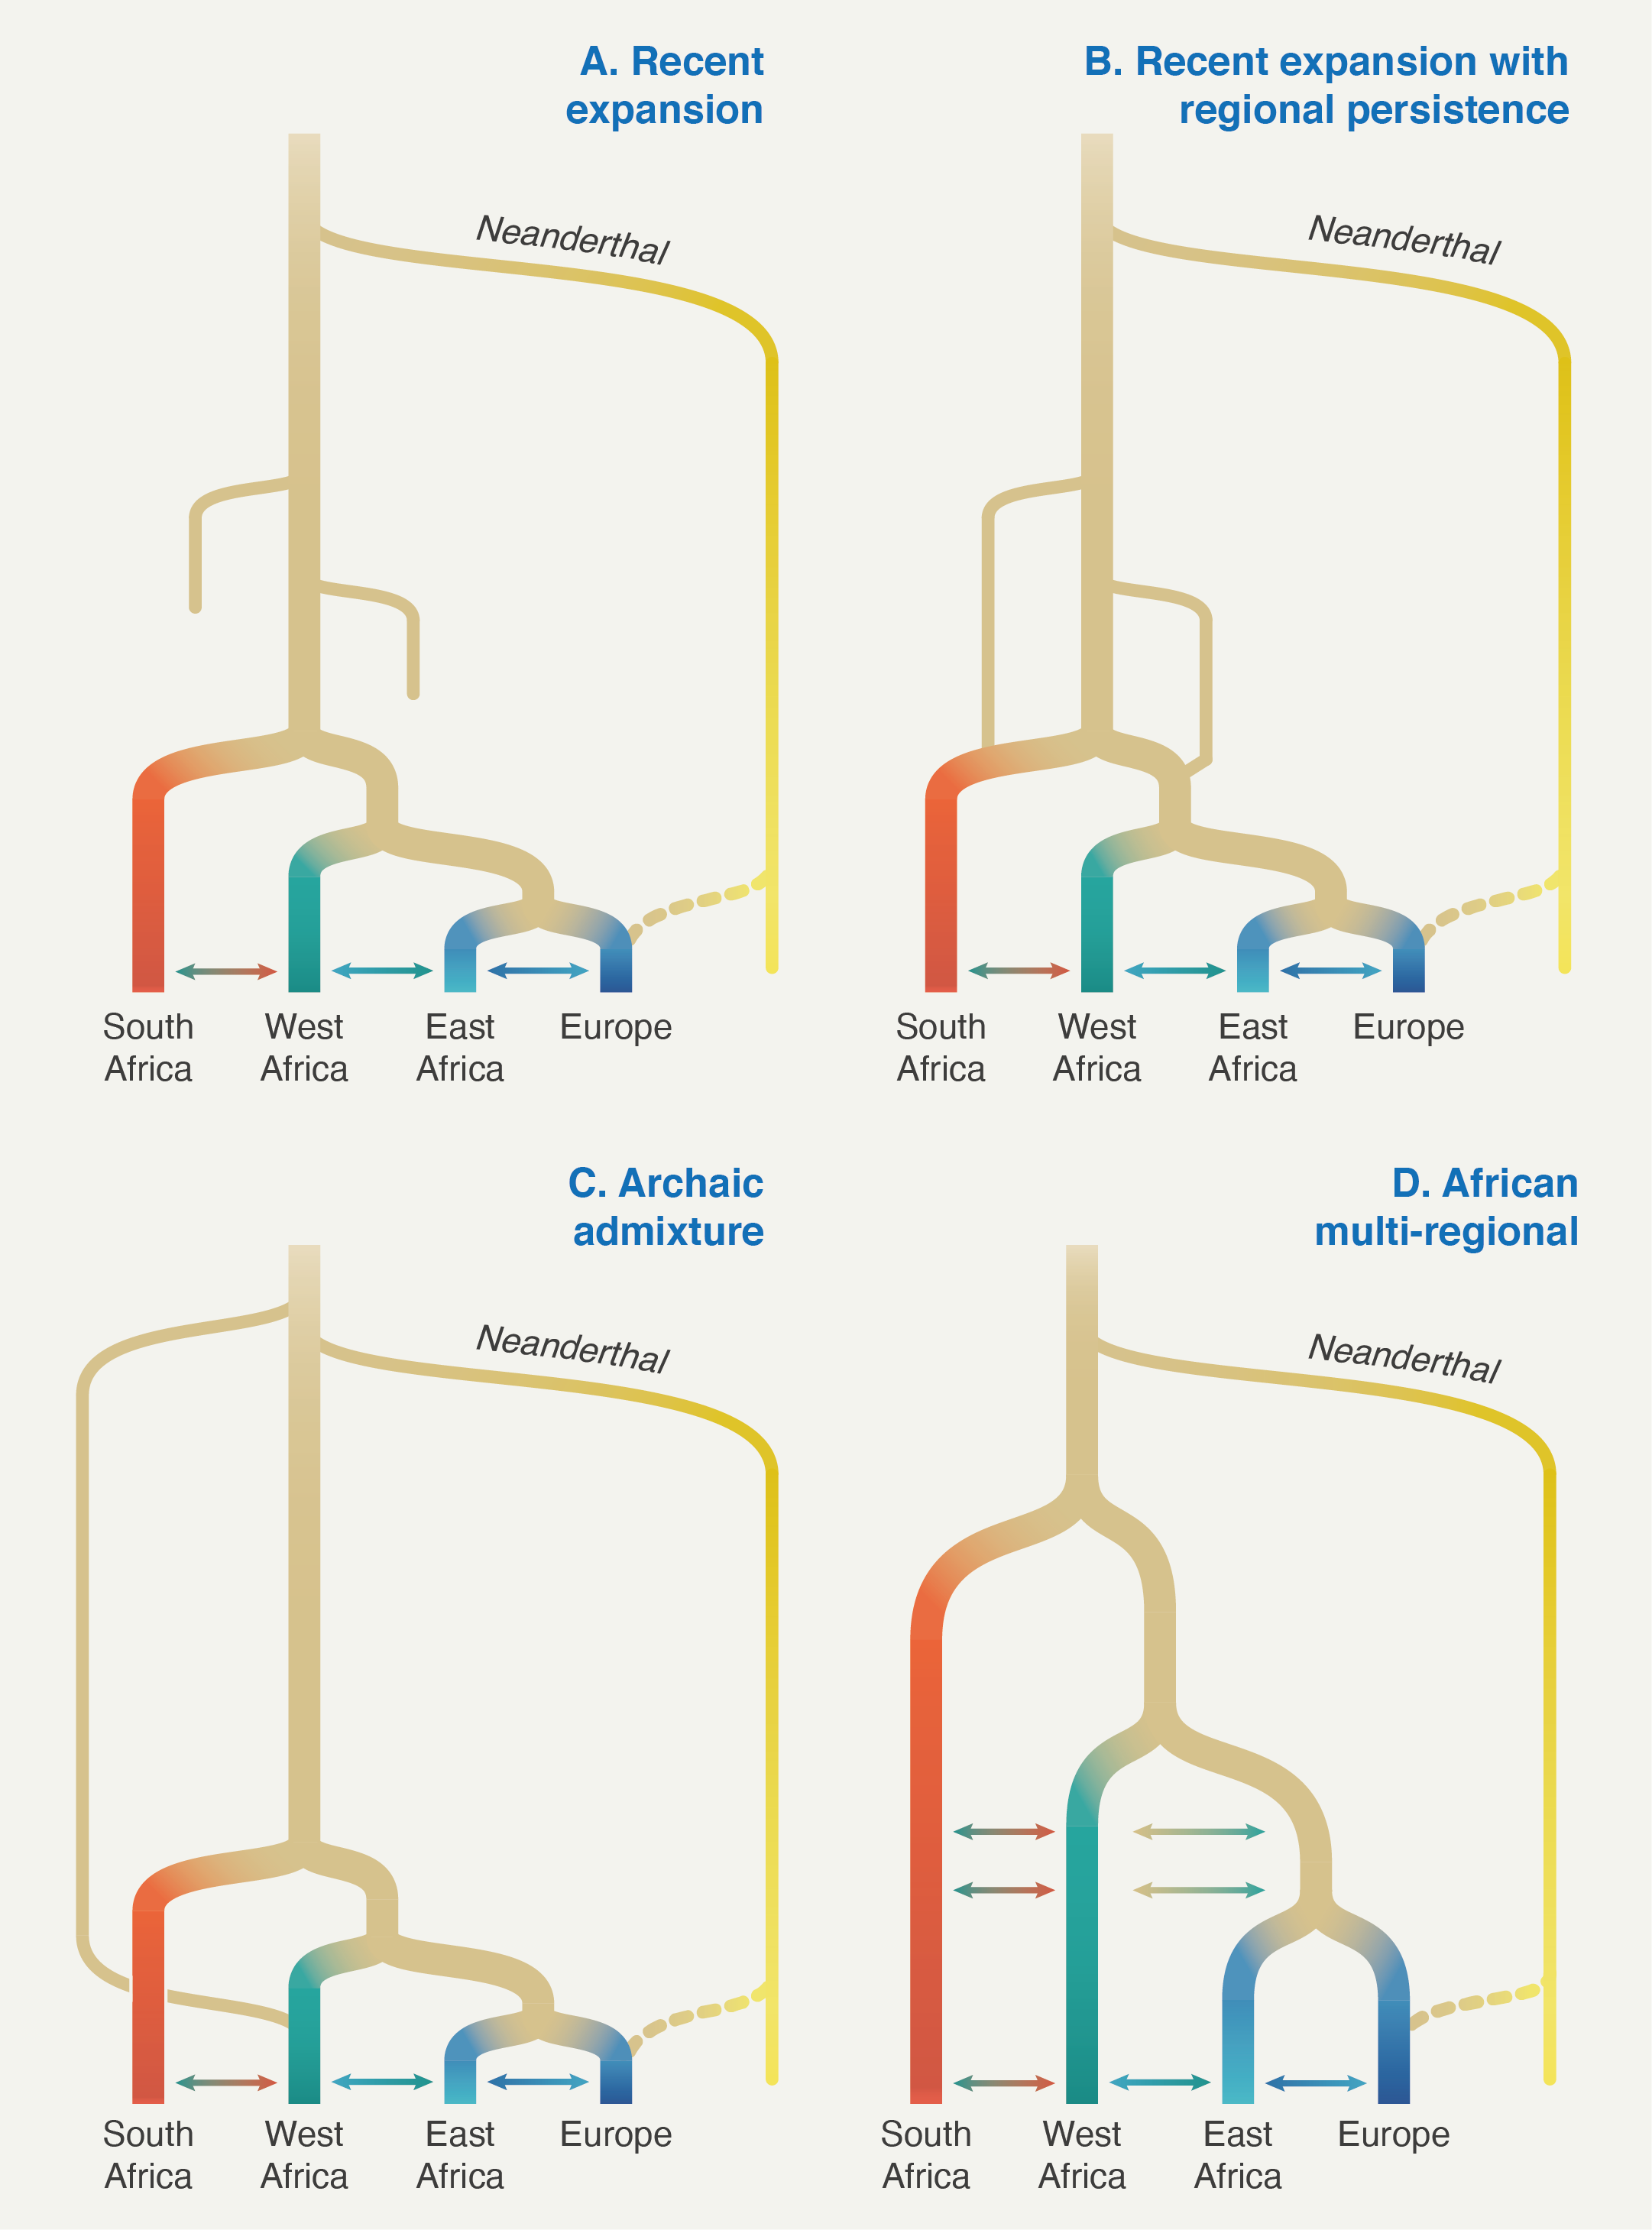
\includegraphics[width=0.5\textwidth]{figures/proposed-models.png}
    \caption{
        \textbf{Proposed conceptual models of early human history in Africa.}
        These models have been designed to translate models from the 
        paleoanthropological literature into genetically testable demographic
        models \citep{Henn2018-rf}.
        We used these conceptual models as starting points to build detailed
        parameterized demographic models (Supp. Information section~\ref{modelspec})
        that were then fit to genetic data. 
    }
    \label{fig:proposed-models}
\end{figure}


\section*{Results}

We inferred detailed demographic histories using 4x-8x whole-genome sequencing
data for four diverse African populations, comprising the Nama (Khoe-San from
South Africa, newly presented here), Mende (from Sierra Leone, MSL from the
Phase 3 1000 Genomes Project \citep{1000_Genomes_Project_Consortium2015-zq}),
Gumuz (recent descendants of a hunter-gatherer group from Ethiopia
\citep{Gurdasani2015-qy,Gopalan2022-pw}), and eastern African agriculturalists
(Amhara and Oromo from Ethiopia \citep{Gurdasani2015-qy}). The Amhara and Oromo
populations, despite speaking distinct Afro-Asiatic languages, are highly
genetically similar \citep{Pagani2015-pz,Gopalan2022-pw} and thus the two
groups were combined for a larger sample size (Figure~\ref{fig:diversity}). We also
included the British (GBR) from the 1000 Genomes Project in our demographic
models as a representative source of back-to-Africa gene flow and recent
colonial admixture in South Africa. Finally, we used a high-coverage ancient
Neanderthal genome from Vindija Cave, Croatia \citep{Prufer2017-kk} to account
for gene flow from Neanderthals into non-Africans and gauge the relative
time depth of divergence, assuming Neanderthals diverged 550ka from a common
stem. We computed one- and two-locus statistics whose expectation within and across 
populations can be computed efficiently and that are well suited for both low- and
high-coverage genomes \citep{Ragsdale2019-nt,Ragsdale2020-nz}. Using a
maximum-likelihood inference framework, we then fit to these statistics a
family of parameterized demographic models that involve population splits, size
changes, continuous and variable migration rates, and punctuated admixture
events, to learn about the nature of population structure over the past million
years.

\begin{figure}[ht!]
    \centering
    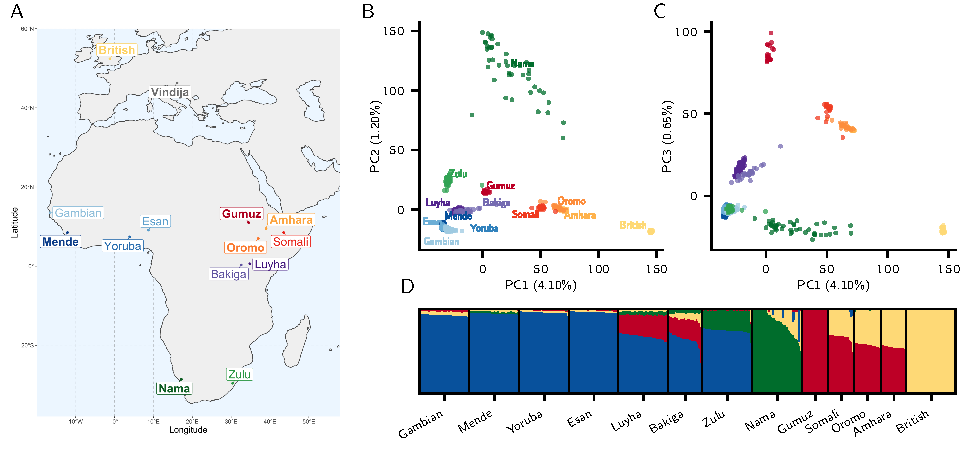
\includegraphics{figures/samples-diversity.pdf}
    \caption[width=\textwidth]{
        \textbf{Genetic diversity across Africa.}
        (A) Select populations from the 1000 Genomes and African Diversity Reference Panels
        illustrate diversity from western, eastern and southern Africa.
        We chose representatives from each region (bold labels)
        to build parameterized models,
        including the newly-sequenced Nama from South Africa, Mende
        from Sierre Leone, Gumuz, Oromo and Amhara from Ethiopia, and the
        British and Vindija Neanderthal individual.
        (B, C) PCA highlights the range of genetic divergence anchored 
        by western Africans, Nama, Gumuz and the British.
        Percentages show variance explained by each principal component.
        (D) \texttt{ADMIXTURE} with $K=4$ illustrates signatures of recent gene flow in Africa
        which reflect colonial-period migration into the Nama,
        Back-to-Africa gene flow among some Ethiopians, and Khoe-San admixture in the Zulu.
    }
    \label{fig:diversity}
\end{figure}
   
\subsection*{A Late Middle Stone Age common ancestry for contemporary humans}

We began with a model of geographic expansion from a single ancestral,
unstructured source followed by migration between populations, without allowing
for contribution from an African archaic hominin lineage or population structure prior
to the expansion (Figure~\ref{fig:proposed-models}A). As expected
\citep{Ragsdale2019-nt}, this first model was a poor fit to the data
qualitatively (Figure~\ref{fig:supp-single-origin-fits}) and quantitatively
(log-likelihood ($LL$) $\approx -189,400$, Table~\ref{tab:supp-single-origin}).
We next explored a suite of models in which population structure predates the
differentiation of contemporary groups, including models allowing for ancestral
reticulation (such as fragmentation-and-coalescence or meta-population models,
Figure~\ref{fig:proposed-models}B), archaic hominin admixture
(Figure~\ref{fig:proposed-models}C), and African multi-regionalism
(Figure~\ref{fig:proposed-models}D).

Regardless of the model choice for early epochs, inference of human demographic
history for the last 150ka was remarkably robust.
In a reticulated model, we use ``divergence'' between populations to describe
the time of their most recent shared ancestry.
The earliest divergence among
contemporary human populations differentiates the southern African Nama from
other African groups between 110--135ka, with low to moderate levels of
subsequent gene flow (Table \ref{tab:migration-rates}). In none of the
high-likelihood models which we explored did the divergence between Nama and
other populations exceed $\sim$140ka. 
We conclude that geographic patterns of contemporary \emph{Homo sapiens} population structure
date back to the late Middle Stone Age in Africa, likely arising during MIS 5.
Although we find evidence for earlier population structure in Africa (see
below), contemporary populations cannot be easily mapped onto the more ancient
`stem' groups as only a small proportion of drift between contemporary populations can
be attributed to drift between stems (Section \ref{sec:f4},  Figures~\ref{fig:predictions} and
\ref{fig:supp-f4s-single-origin}--\ref{fig:supp-f4s-merger-with-stem-migration}). 

Given this consistency in inferred recent history and the numerical challenge
of optimizing a large number of parameters, we fixed several parameters related
to recent population history so as to focus on more ancient events. 
Fixed parameters included
the time of divergence between western and eastern African populations,
set to 60ka, just prior to the split of Eurasians and East Africans set to 50ka. 
We also fixed the amount of admixture from Neanderthals to Europeans directly
following the out-of-Africa migration which was set to 1.5\% at 45ka (Supp. Information).
These constraints allowed us to integrate information from previous genetic
and archaeological research to infer robust migration rates.
For example, all models infer relatively high gene flow between Ethiopia and western Africa
($m\approx2\times10^{-4},$ the constant proportion of migrant lineages per generation over 60ka).
We further find that Back-to-Africa gene flow at the beginning of the Holocene primarily
affected the ancestors of the Ethiopian agricultural populations, comprising
over half of their genetic ancestry, estimated to be 64--65\%. The past 5,000
years also saw major demographic changes, including strong population growth
for western Africans as they specialized in yam and oil palm agriculture
(estimated 3-fold growth). We observe significant gene flow from the Amhara and
Oromo into the Nama, a signal which is likely a proxy for the movement of
eastern African caprid and cattle pastoralists
\citep{Henn2008-xo,Breton2014-xb}, here estimated to constitute a 25\% ancestry
contribution 2,000 ya. Colonial period admixture from Europeans into the Nama
was estimated at 15\%, similar to proportions suggested by \texttt{ADMIXTURE}
(Figure~\ref{fig:diversity}).

\begin{figure}[t!]
    \centering
    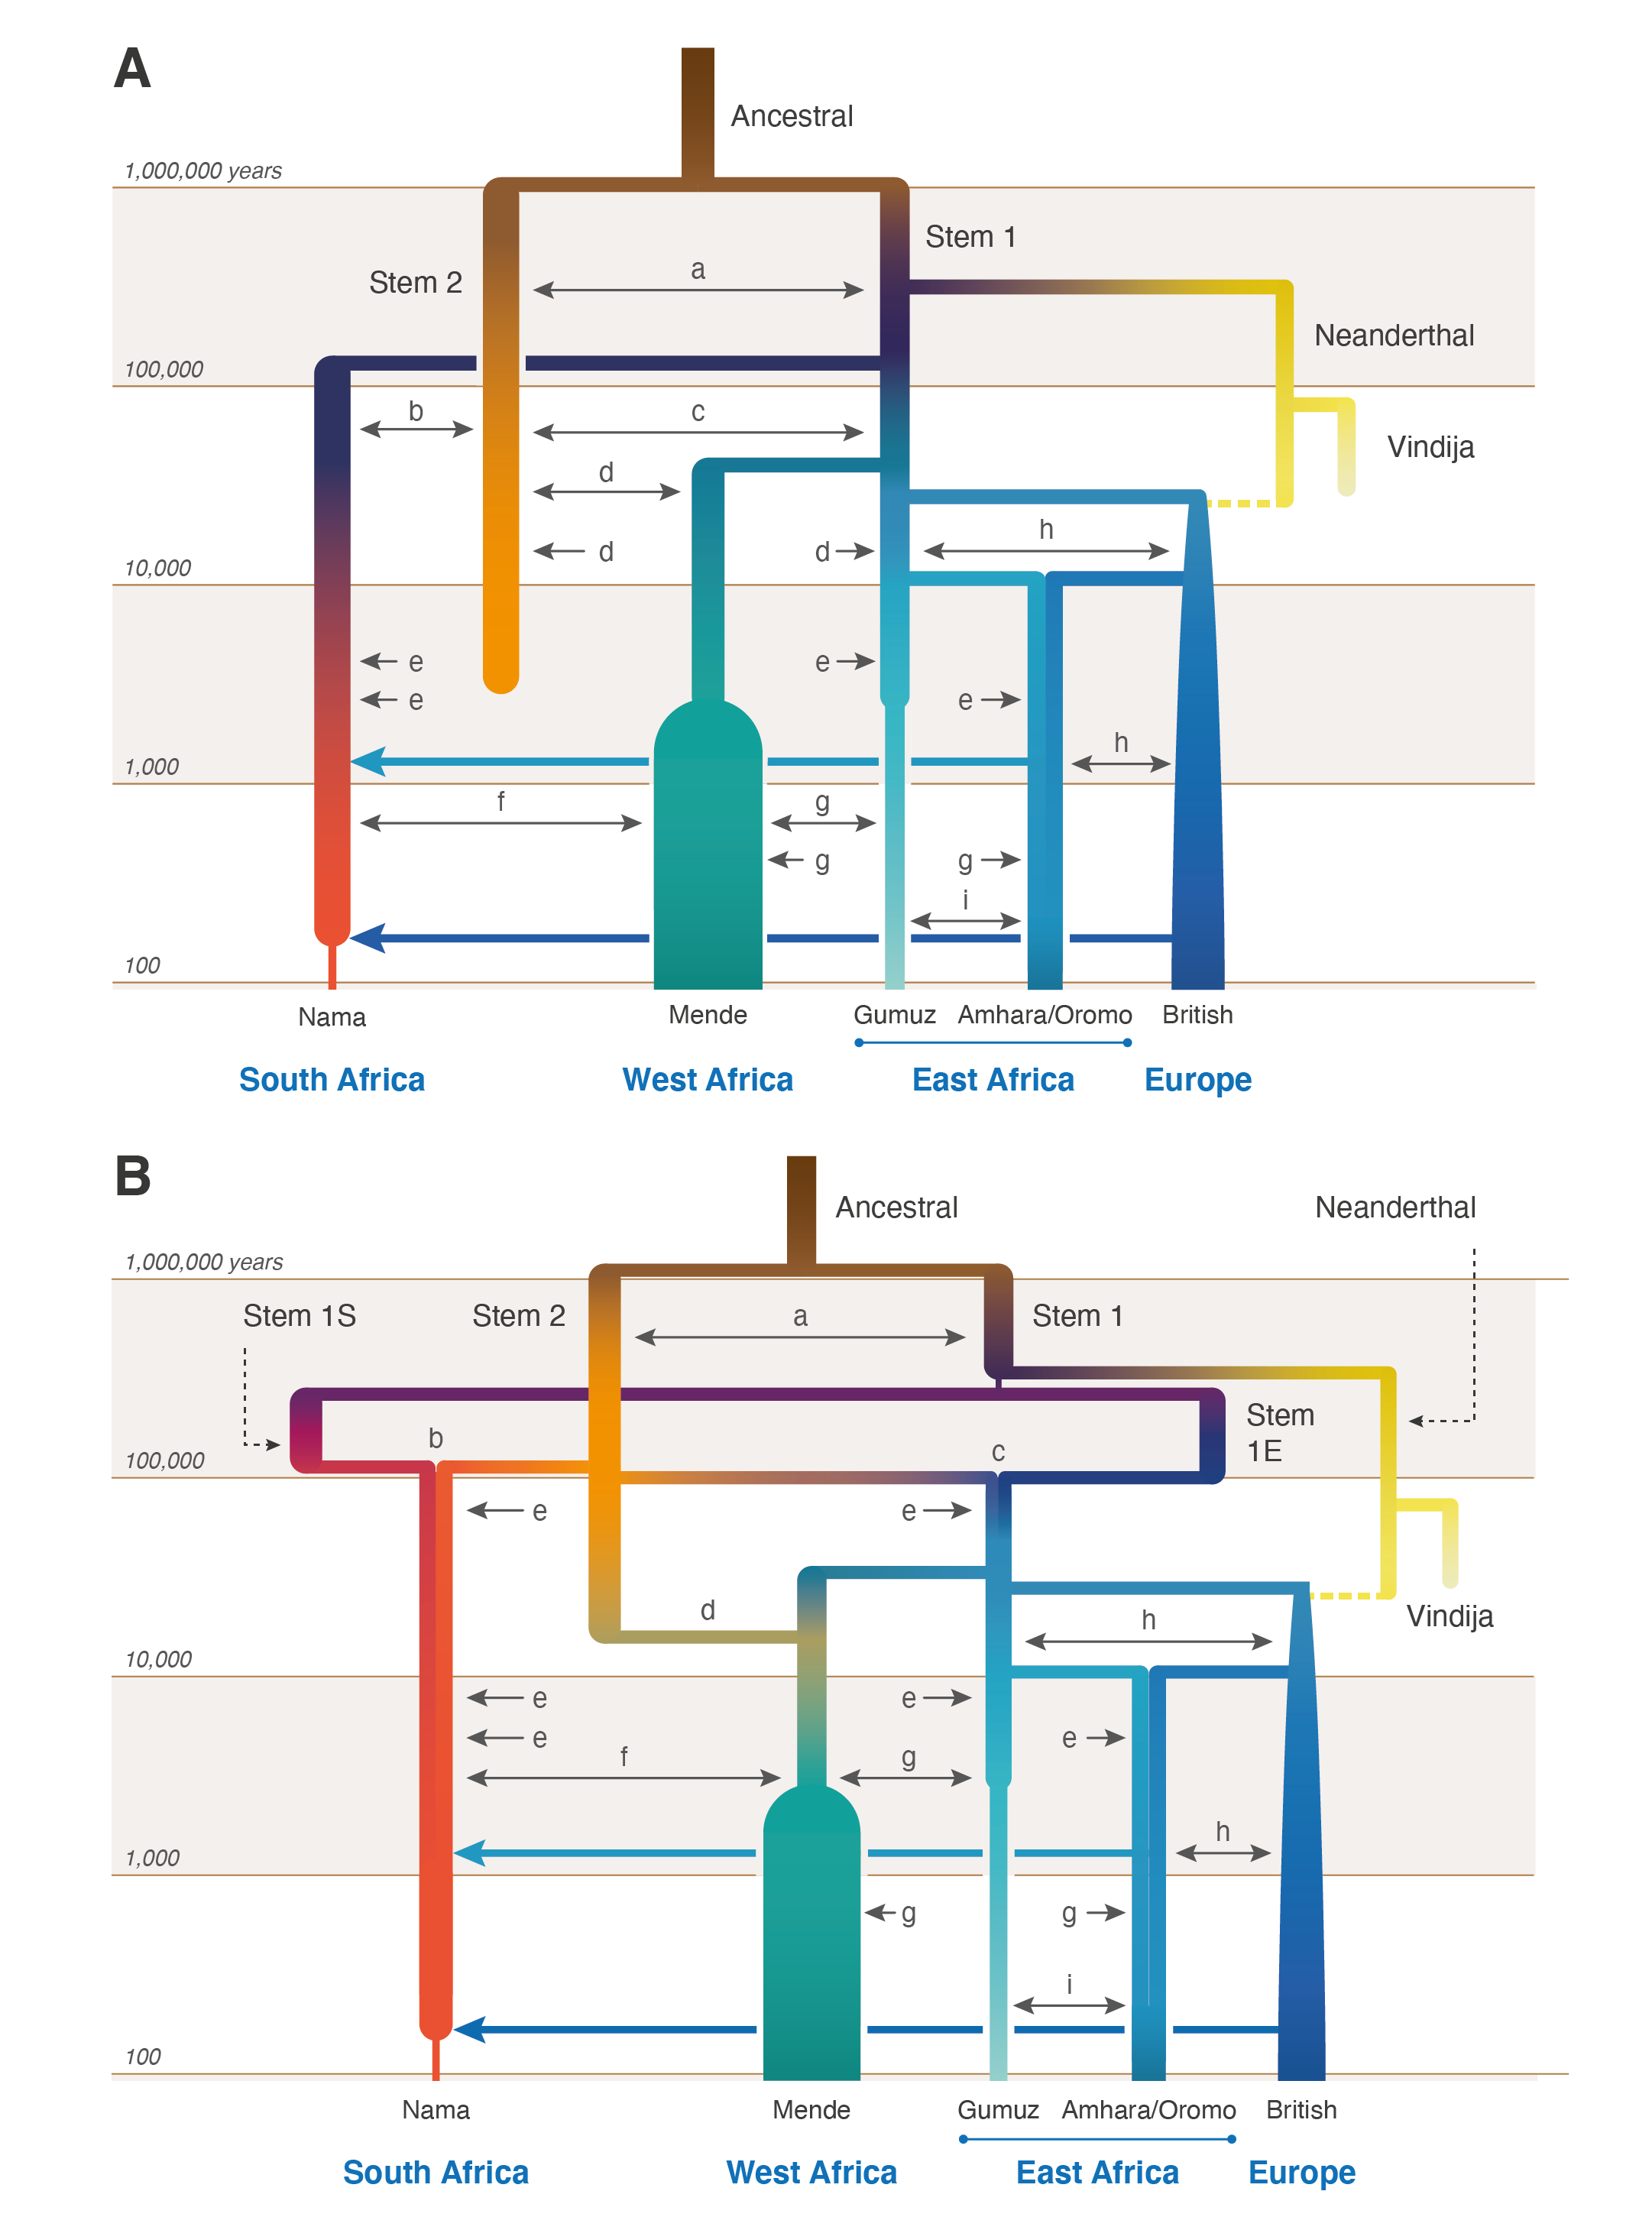
\includegraphics[width=0.65\textwidth]{figures/best-fit-models}
    \caption{
        \textbf{A weakly structured stem best describes two-locus statistics.}
        In the two best-fitting parameterizations of early population structure,
        continuous migration (A) and multiple mergers (B), models
        that include ongoing migration between stem populations outperform
        those in which stem populations are isolated. Most recent populations are
        connected by continuous, reciprocal migration that are indicated by 
        double-headed arrows (labels matched to migration rates and divergence
        times in Table~\ref{tab:migration-rates}). These migrations last for the
        duration of co-existence of contemporaneous populations with constant
        migration rates over those intervals. The
        merger-with-stem-migration model (B, with  $LL=-102,600$) outperformed the
        continuous-migration model (A, with $LL=-115,500$ ).
        Colors are used to distinguish overlapping branches and link to
        Figure~\ref{fig:diversity}.}
    \label{fig:best-fit-models}
\end{figure}

\begin{table}[t!]
    \centering
    \scriptsize
    \begin{tabular}{lllrrrr}
        \toprule
        \textbf{Likelihood} & \textbf{Label} & \textbf{Population Pair} &
            \textbf{Divergence} & \textbf{Migration rate} & \textbf{Migration} \\
        & & & 
            \textbf{Time (ka)} & \textbf{per generation} & \textbf{duration (kyr)} \\
        \midrule
        \textbf{Continuous Model} & & & & & \\
        $LL= -115,500$ & a & Stem 1, Stem 2 & 1,163 & 6.43e-5 & 1,028 \\
        (Table~\ref{tab:supp-continuous-migration}) & b & Stem 2, Nama & NA & 5.82e-5 & 130 \\
        & c, d & Stem 2, Other Africans* & NA & 3.10e-5, \textbf{1.64e-4} & 130, 55 \\
        & e, f & Nama, Other Africans* & 135 & 4.1e-5, 9.8e-6 & 135, 60 \\
        & g & Mende, East Africans & 60 & \textbf{2.14e-4} & 60 \\
        & h & East Africans, British & 50 & 4.17e-5 & 50 \\
        & i & Gumuz, Amhara/Oromo & 12 &\textbf{3.36e-4} & 12 \\
        \textbf{Merger Model} & & & & & \\
        $LL= -102,600$ & a & Stem 1, Stem 2 & 1,442 & \textbf{1.16e-4} & 963 \\
        (Table~\ref{tab:supp-merger-with-stem-migration}) & -- & Stem 1S, Stem 1E & 479 & 0 (fixed) & -- \\
        & b & Stem 2 to Nama & 119 & \textbf{0.71} & pulse \\
        & c & Stem 2 to Stem 1E & 98 & \textbf{0.50} & pulse \\
        & d & Stem 2 to Mende & 25 & \textbf{0.18} & pulse \\
        & e, f & Nama, Other Africans* & 119 & 4.4e-5, 7.1e-6 & 119, 60 \\
        & g & Mende, East Africans* & 60 & \textbf{1.98e-4} & 60 \\
        & h & East Africans, British & 50 & 3.87e-5 & 50 \\
        & i & Gumuz, Amhara/Oromo &12 & \textbf{3.59e-4} & 12 \\
        \bottomrule
    \end{tabular}
    \caption{
        \textbf{Migration and divergence parameters from best fit models.}
        Labeled migration rates correspond to symmetric continuous migration
        bands shown in Figure~\ref{fig:best-fit-models}. Both the continuous migration and
        merger models inferred a relatively deep split of human stem branches,
        though they were connected by ongoing migration that maintained their
        genetic similarity. Bold text indicates migration rates above $10^{-4}$.
        In both models, the branch ancestral to the Nama shares a common ancestral population
        with the other African groups $\sim$120--135ka. Following this divergence,
        the population ancestral to other African groups branches into West and East African
        groups 60ka.
        *Migration rates and durations are shown between branches ancestral to 
        1) Nama and East Africans and their ancestors, and
        2) Nama and Mende, respectively.
        ``Divergence times'' correspond to the most recent common ancestral population,
        and does not account for continuous migration or earlier reticulations.
    }
    \label{tab:migration-rates}
\end{table}

\subsection*{Deep but connected population structure within Africa}

To account for population structure prior to 135ka, three of our four models allowed for two or more
``stem'' populations which could diverge either before or after the Neanderthal
split. We considered models both with and without migration between these stem
populations, and in both cases we tested two different types of gene exchange
during the expansion phase, as illustrated in Figure \ref{fig:mergers}:
1) One of the stem population expands (splits into
contemporary populations), and the other stem population(s) has continuous
symmetric migration with those populations; or 2) one or more of the stem
populations expands, with instantaneous pulse (or ``merger'') events from the
other stem population, so that recent populations are formed by mergers
of multiple ancestral populations. Depending on parameter values,
this scenario encompasses archaic hominin introgression and
fragmentation-and-coalescence models (such as Figure~\ref{fig:proposed-models}B and C).
For many parameters, confidence intervals based on bootstrapping are relatively narrow
(Tables~\ref{tab:supp-single-origin}--\ref{tab:supp-merger-with-stem-migration}),
reflecting an informative statistical approach. Model assumptions
have, however, a larger impact on parameter estimates (and thus, real uncertainty).
To convey model uncertainty, we highlight features of the two inferred models
with high likelihoods. These are referred to as the
``multiple-merger'' and the ``continuous-migration'' models. Both allow for
migration between stem branches, but differ primarily in the timing of the
early divergence of stem populations and their relative $N_e$
(Figure~\ref{fig:best-fit-models}). The two models also differ in the mode of divergence
during the Middle Stone Age.

Allowing for continuous migration between the stem populations substantially
improved the fits relative to zero migration between stems
($LL \approx -102,600$ vs. $-107,700$ in the merger model and
$LL \approx -115,500$ vs. $-126,600$ in the continuous migration model).
With continuous migration between stems, population
structure extends back to 1.1--1.4Ma (Table~\ref{tab:migration-rates}).
Migration between the stems in these models is moderate, with a fraction of
migrant lineages each generation estimated as
$m=6.4\times10^{-5}-1.2\times10^{-4}$. For comparison, this is similar
to inferred migration rates between connected contemporary populations over the
past 50ka (Table~\ref{tab:migration-rates}). This ongoing (or at least,
periodic) gene flow qualitatively distinguishes these models from previously
proposed archaic hominin admixture models (Figure~\ref{fig:proposed-models}C) as
the early branches remain closely related, and each branch contributes large
amounts to all contemporary populations (Figure~\ref{fig:predictions}). 
Because of this relatedness, only $1\%$ to $4\%$ of genetic differentiation
among contemporary populations can be traced back
to this early population structure (Supp. Information)
 
Under the continuous-migration model, one of the two stems diverges into
lineages leading to contemporary populations in western, southern and eastern
Africa, and the other (Stem 2) contributes variable ancestry to those
populations. This migration from Stem 2 is highest with the Mende
($m=1.6\times10^{-4}$) compared to the Nama and East African populations
($m=5.8\times10^{-5}$ and $3.1\times10^{-5}$, respectively), with migration
allowed to occur until 5ka. A
sampled lineage from the Nama, Mende, and Gumuz have probabilities of being in
Stem 2 at the time of Stem 1 expansion (135ka) of approximately $0.145$, $0.2$,
and $0.13$, respectively, though these probabilities change over time,
precluding the notion of a fixed admixture proportion.

In contrast, under the multiple-merger model, stem populations merge with
varying proportions to form the different contemporary groups. 
We observe a sharp bottleneck in Stem 1 down to $N_e=117$ after the split of
the Neanderthal branch. This represents the lower bound allowed in our
optimization (i.e. 1\% of the ancestral $N_e$), although the size of this
bottleneck is poorly constrained ($\sigma_{N_e}=838$). After a long period of
exchange with Stem 2, Stem 1 then fractures into ``Stem 1E'' and ``Stem 1S''
479ka. The timing of this divergence was also poorly constrained ($\sigma_T=
166$ka). These populations evolve independently until 119ka
($\sigma_T=
28$ka) when Stem 1S and Stem 2 combine to form the ancestors of the Nama, with
proportions 29\%, 71\% respectively. Similarly, Stem 1E and Stem 2 combine in
equal proportions (50\% each) to form the ancestors of the western Africans and
eastern Africans (and thus also all individuals who later disperse during the
Out of Africa event). Finally, the Mende receive a large additional pulse of
gene flow from Stem 2, replacing 18\% of their population 25ka ($\sigma_T=
0.6$ka).
The later Stem 2 contribution to the western African Mende resulted in
better model fits ($\Delta LL \approx 60,000$).
Speculatively, this may indicate that an ancestral Stem 2 population occupied western or
Central Africa, broadly speaking. The differing proportions in the Nama and
eastern Africans may also indicate geographic separation of Stem 1S in southern
Africa and Stem 1E in eastern Africa. 

\begin{figure}[t!]
    \centering
    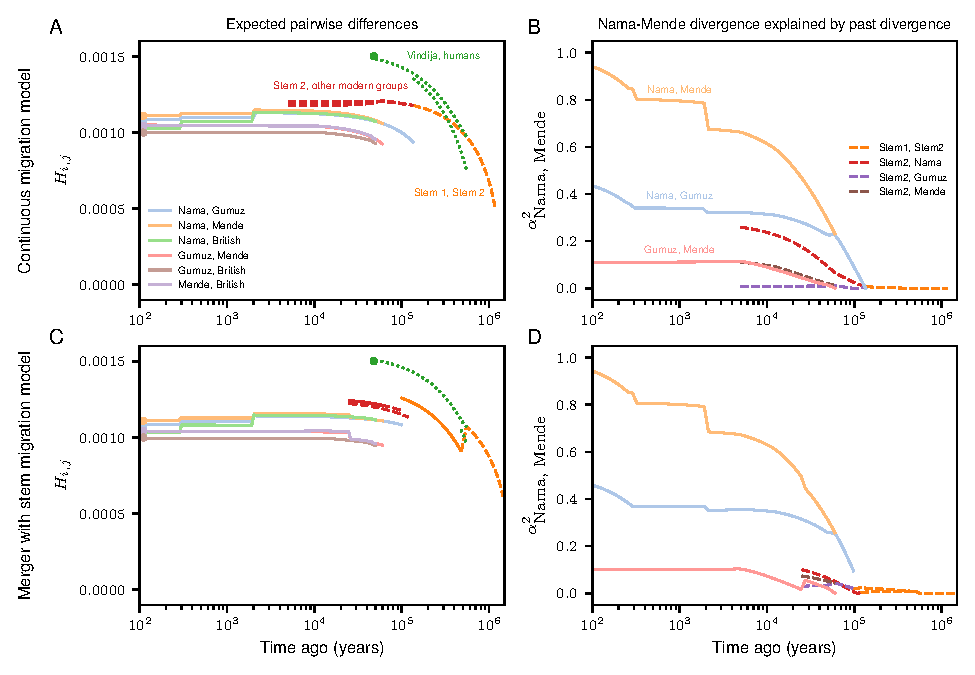
\includegraphics{figures/predictions.pdf}
    \caption{
        \textbf{Structure among stems is weak and present-day structure is mostly recent.}
        From the best fit models of our two parameterizations (A and B:
        continuous migration, C and D: merger with stem migration),
        we predicted pairwise differences $H_{i,j}$ between individuals
        sampled from populations $i$ and $j$ existing at time $t$ (A and C).
        (B and D) To understand how drift between stems explains contemporary structure, 
        we also computed the proportion $\alpha^2$ of drift between pairs of
        sampled contemporary
        populations that aligns with drift between past populations
        (here Nama and Mende, see Section~S\ref{sec:f4} for details and additional
        comparisons in Figures~\ref{fig:supp-f4s-single-origin}--\ref{fig:supp-f4s-merger-with-stem-migration}).
        Both models infer deep population structure with modest contributions to
        contemporary genetic differentiation.
        Most present differentiation dates back to the last 100ka.
    }
    \label{fig:predictions}
\end{figure}

\subsection*{Reconciling multiple lines of genetic evidence}

Previous studies have found support for archaic hominin admixture in Africa using
two-locus statistics \citep{Hsieh2016-gk,Ragsdale2019-nt}, the conditional SFS
(cSFS) \citep{Durvasula2020-td}, and reconstruction of gene genealogies
\citep{Speidel2019-nj}. However, none of these studies considered a weakly
structured stem. We validated our inferred models with additional independent
approaches. We find that the observed cSFS (conditioned on the derived allele
being carried in the Neanderthal sample) is very well-described by the merger
model (Figures~\ref{fig:validation}A-C and
\ref{fig:supp-csfs-single-origin}--\ref{fig:supp-csfs-merger-with-stem-migration}),
even though this statistic was not used in the fit. Our best-fit models outperform
archaic hominin admixture models fit directly to the cSFS
(for example, compare to Figure~1 in
Durvasula and Sankararaman (2020)\citep{Durvasula2020-td}).

\begin{figure}[t!]
    \centering
    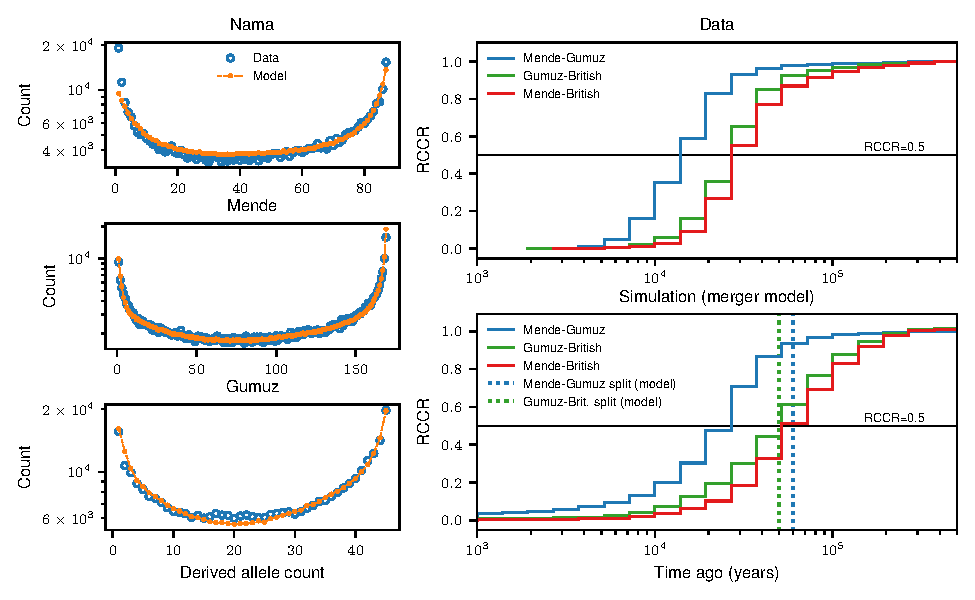
\includegraphics{figures/validation}
    \caption{
        \textbf{Model validation using independent statistics.} (A--C) Using
        our best fit models to linkage disequilibrium and pairwise diversity statistics,
        we simulated expected conditional site-frequency-spectra (cSFS) and
        compared to the observed cSFS from the data. Our inferred models
        provide a good fit to the data, even though these were not used in our
        inference. Across the three populations, ancestral state
        misidentification was consistently inferred to be 1.5--1.7\% for
        intergenic loci (Supp. Information). (D, E) We used Relate
        \citep{Speidel2019-nj} to reconstruct genome-wide gene genealogies,
        which we used to estimate coalescence rate trajectories and
        and cross-coalescence rates between pairs of populations. While
        coalescence rate distributions are informative statistics about past
        evolutionary processes, interpretation can be hindered by migration and
        population structure, and translating relative cross-coalescence rate
        curves (RCCR) into population divergence times is especially prone
        to misinterpretation. For example, the Mende-Gumuz comparison shows
        a more recent increased RCCR than either population with the British,
        a pattern that is recapitulated under our best-fit model, even though
        the Mende-Gumuz split occurs prior to the Gumuz-British split.
    }
    \label{fig:validation}
\end{figure}

We used \texttt{Relate} \citep{Speidel2019-nj} to infer the distribution of
coalescence rates over time in real data and data simulated from our inferred
models. Many previous studies have found a reduction of coalescence rates
between $1000$ka and $100$ka in humans, and thus inferred an increase in $N_e$
during the same period \citep{Li2011-le}.  This increase in inferred $N_e$
could be due to either an increase in population size or to ancestral
population structure during the Middle Stone Age \citep{Mazet2016-wn}.  All
models, including the single-origin model, recapitulate an inferred ancestral
increase in $N_e$ between 100ka-1Ma extending deeper in the past than the
relate estimate (Figure~\ref{fig:supp-iicr-sim} and Section
\ref{inferred_relate}). Whereas the single-origin model achieves this by an
increase in $N_e$ during that period, the best-fit model recapitulate this
pattern without corresponding population size changes.     

Relative cross-coalescence rates (rCCR) have recently been used to estimate
divergence between a pair of populations, as measured by the rate of
coalescence between two groups divided by the mean within population
coalescence. Simulations of rCCR accuracy, however, focus on a ‘clean split’
between populations whereby groups diverge without subsequent gene flow.
Published estimates of the earliest human divergences with rCCR, which range
from 150ka-100ka \citep{Bergstrom2021-iw}, may be significantly biased when
compared to more complex models with gene flow as inferred here. We find that
midpoint estimates of rCCR are poor estimates for population divergence, often
underestimating divergence time by 50\% or greater (e.g., Mende vs. Gumuz
$\sim$15ka compared to a true divergence of 60ka), and recent migration can
lead to the misordering of divergence events (Figure~\ref{fig:validation}E). We
suggest that rCCR analyses which do not fit multiple parameters including gene
flow should be interpreted with caution.

Other studies have fit tree-like demographic models to African populations
using distributions of allele frequencies or related statistics, finding
inconsistent divergence times \cite{Henn2018-rf,Bergstrom2021-iw}.
Section~\ref{sec:IM-reinfer} explains this behaviour: split times inferred
using isolation with migration models and distributions of allele frequencies
simulated under our reticulated models are highly variable and much deeper than
the more recent estimated population divergence. 

\section*{Discussion}

Any attempt at building detailed models of human history is subject to model
misspecification. This is true of earlier studies, which often assumed that
data inconsistent with a single-origin model must be explained by archaic
hominin admixture. This is also true of this study. While it remains prohibitive to
fully explore the space of plausible models of early human population structure,
we sought to capture model uncertainty by exploring multiple parameterizations of
early history.
The best-fit models presented here include reticulation and migration between
early human populations rather than archaic hominin admixture from long-isolated branches.
We cannot rule out that more complex models involving
additional stems, continuous structure, or hybrid models including both weak structure and archaic
hominin admixture may better explain the data. Because parameters related to the split
time, migration rates, and relative sizes of the early stems were variable
across models, reflecting a degree of confounding among these parameters, we
refrained from introducing additional branches associated with more
parameters during that period.
Rather than interpreting the two stems as representing well-defined
and stable populations over hundreds of thousands of years, we interpret the
weakly structured stem as consistent with a population coalescence and
fragmentation model \citep{Scerri2019-xg}.
Models including additional diversity within Africa,
and early ancient DNA samples from Africa, could further distinguish
the archaic hominin admixture model from the weakly-structured-stem model.

\subsection*{The Middle Stone Age in Africa}

By contrast, our inferred models paint a more consistent picture of the late
Middle Stone Age as a critical period of change, assuming that estimates from
the recombination clock accurately relate to geological chronologies
(Supp. Information).
During the Middle Stone Age, the multiple merger model indicates three
major stem lineages in Africa, tentatively assigned to southern (Stem 1S),
eastern (Stem 1E) and western/central Africa (Stem 2). While the length of
isolation among the stems is variable across model fits, models with a period of 
divergence, isolation and then a merger event (i.e. a ``reticulation''
out-performed models with bifurcating divergence and continuous gene flow. 

A population reticulation involves multiple stems contributing genetically to
the formation of a group. One way in which this can happen is through the
geographic expansion of one or both stems. For example, if during MIS 5, either
Stem 1S (Figure~\ref{fig:best-fit-models}B) 
from southern Africa moved northward thereby encountering Stem 2,
or Stem 2 moved from central/western Africa southward into Stem 1S -- then we
could observe disproportionate ancestry contributions from different stems in
contemporary groups. We observed two merger events. The first, between Stem 1S and
Stem 2, results in the formation of an ancestral Khoe-San population $\approx120$ka.
The second $\approx100$ka between Stem 1E and Stem 2, results in the formation of the
ancestors of East/West Africans as well as later ``Out of Africans''. The rapid
rise in sea levels and increased precipitation during MIS 5e, following a
glacial period of aridity across Africa \citep{Blome2012-lw}, might have
triggered migration inland away from the coasts, as has been suggested, e.g., for the
Paleo-Agulhas plain \citep{Marean2014-pg}.


Following these merger events, the stems subsequently fracture into
subpopulations which then appear to persist over the past $\sim120$ka. These
subpopulations can be linked to contemporary groups despite subsequent gene flow
across the continent; for example, a genetic lineage sampled in the Gumuz has a
$0.44$ probability of being inherited from the ancestral ‘eastern’ subpopulation
(Stem 1E) 150ka versus $0.03$ probability of being inherited from the ‘southern’
subpopulation (Stem 1S) and $0.53$ probability of being inherited from Stem 2
(see Table~\ref{tab:supp-lineage-probabilitys} for additional comparisons). We also
find that Stem 2 continued to contribute to western Africans during the Last
Glacial Period, indicative that this gene flow likely occurred in
western/central Africa (Table~\ref{tab:migration-rates}). 



\subsection*{Contrasting archaic hominin admixture and a weakly structured stem}

Evidence for archaic hominin admixture in Eurasia has bolstered the plausibility of 
archaic hominin admixture having also occurred in Africa. For this reason, previous 
work has focused on archaic hominin admixture to explain patterns of polymorphism 
inconsistent with a single-origin model. Here, we have shown that weakly-structured-stem 
models better capture these patterns. Preferring weakly-structured-stem models over 
archaic-admixture models potentially has ecological implications. With a weakly 
structured stem, there is no need to posit that an archaic hominin population stayed 
reproductively isolated from the ancestral human lineage for thousands of years before 
the initiation of gene flow. Instead, there would have been continuous or recurrent 
contact between two or more groups present in Africa. It would be fruitful to 
investigate the ecological reasons for continued contact between groups within Africa 
but long periods of isolation between African and Eurasian groups.

There is evidence for both deleterious and adaptive archaic-hominin-derived alleles in
contemporary genomes in the form of a depletion of Neanderthal ancestry in regulatory
regions \citep{Petr2019-xo} or an increased frequency of archaic-hominin-related
haplotypes such as at \emph{EPAS1} among Tibetans \citep{Zhang2021-xx}. Under previous
African archaic hominin admixture models, the estimated 8--10\% introgression rate is
much higher than Neanderthal gene flow, and would have plausibly been fertile
ground for dramatic selection for or against archaic-hominin-derived haplotypes\citep{Wall2019-ao}. By contrast, adaptation under a weakly
structured stem would have occurred continuously over much longer periods.
Patterns of polymorphism that are inconsistent with the single-stem model
predictions have been used to infer putative archaic admixed segments
\citep{Plagnol2006-lt,Hsieh2016-gk,Wall2019-ao,Durvasula2020-td}, negative
selection against such segments \citep{Wall2019-ao}, and pervasive positive
selection \citep{Schrider2017-kl}. However, such approaches are subject to high
false positives in the presence of population structure with migration
\citep{Petr2019-xo}, and their interpretation should be re-examined in light of
a weakly-structured-stem model within Africa. 

Multiple studies have shown a correspondence between phenotypic
differentiation, usually assessed with measurements of the cranium, and genetic
differentiation among human populations and between humans and Neanderthals
\citep{Relethford1994-mh,Weaver2008-ho,Von_Cramon-Taubadel2009-zb}
(see also Section \ref{sec:morpho_diff}).
This correspondence allows predictions of our model to be related to the fossil record.
The fossil record of Africa is sparse during the time period of the stems, but of the
available fossils, some are very similar in morphology to contemporary humans
(e.g., from Omo Kibish, Ethiopia \citep{Day1969-rh,Vidal2022-qe}),
others are similar in some morphological features but not others
(e.g., from Jebel Irhoud, Morocco \citep{Hublin2017-cq,Richter2017-zu}),
and others are very different in morphology
(e.g., from Dinaledi, South Africa \citep{Berger2015-bq,Dirks2017-uk}).
If, as our model predicts, the
genetic differences between the stems were comparable to those among
contemporary human populations, the most morphologically divergent fossils are unlikely to
represent branches that contributed appreciably to contemporary human
ancestries.

\section*{Acknowledgements}

We are grateful for the DNA contribution from each participant which enabled
this study; in particular we wish to highlight the generous participation of
the Richtersveld Nama community in South Africa and help from local research
assistants Willem DeKlerk and Hendrik Kaimann. Additional assistance and
community engagement was conducted by Justin Myrick, Chris Gignoux, Caitlen
Uren and Cedric Werely. We thank the African Genome Diversity Project for data
generation, including Tommy Carensten, Deepti Gurdasani, and Manj Sandhu. We
thank Luke Anderson-Trocm\'e for assistance in creating the map in
Figure~\ref{fig:diversity}. This research was supported by an NIH grant R35GM133531 (to
BMH). The content is solely the responsibility of the authors and does
not necessarily represent the official views of the National Institutes of
Health.

\bibliographystyle{naturemag}
\bibliography{paper}
\end{document}
